\label{sec:chainreader}

In Section \ref{splitting-traj} we showed how splitting the trajectories would help to overcome I/O and improve scaling. 
However, the number of trajectories may not necessarily be equal to the number of processes.
For example, trajectories from MD simulations on HPC machines are often kept in small chunks that need to be concatenated to form a trajectory that can be analyzed with the typical tools.
For the subfiling (splitting trajectories) such chunks might be useful but making sure that the number of processes is equal to the number of trajectory files will not always be feasible for the typical users. 
\package{MDAnalysis} can transparently represent multiple trajectories as one virtual trajectory using the ``ChainReader''.
This feature is already very convenient for serial analysis when trajectories are maintained as chunks.
In the current implementation of ChainReader, each process opens all the trajectories but I/O will only happen from a specific block of the trajectory specific to that process only.

We wanted to test if the ChainReader would benefit from the gains measured for the subfiling approach.
Specifically, we measured if the MPI-parallelized RMSD task (with $N_{\text{p}}$ ranks) would benefit if the trajectory was split into $N_{\text{seg}} = N_{\text{p}}$ trajectory segments, corresponding to an ideal scenario.
 
 \begin{figure}[ht!]
\centering
\begin{subfigure}{.3\textwidth}
  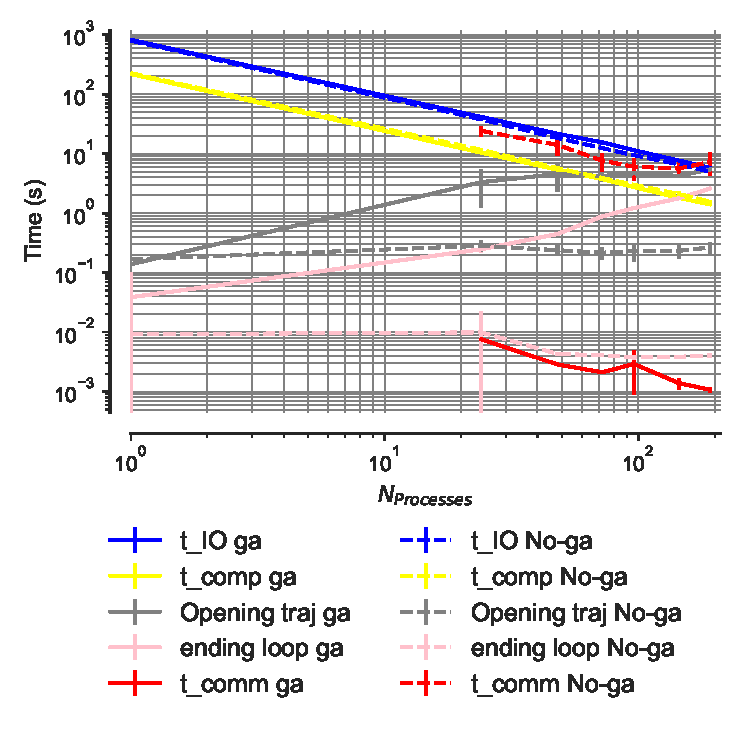
\includegraphics[width=\linewidth]{figures/Comparison_IO_compute_scaling_traj_splitting-chain-reader.pdf}
  \captionsetup{format=hang}
  \caption{Scaling for different components}
  \label{fig:MPIscaling-chain-reader}
\end{subfigure}
\hfill
\begin{subfigure}{.3\textwidth}
  \includegraphics[width=\linewidth]{figures/Comparison_tot_time_traj_splitting-chain-reader.pdf}
  \caption{Scaling total}
  \label{fig:MPItottime-chain-reader}
\end{subfigure}
\hfill
\begin{subfigure}{.3\textwidth}
  \includegraphics[width=\linewidth]{figures/Comparison_Speed_UP_traj_splitting-chain-reader.pdf}
  \caption{Speed-up}
  \label{fig:MPIspeedup-chain-reader}
\end{subfigure}
\bigskip

\begin{subfigure} {.45\textwidth}
  \includegraphics[width=\linewidth]{figures/chain-reader-no-ga-BarPlot-rank-comparison_192_5.pdf}
  \captionsetup{format=hang}
   \caption{Time comparison on different parts of the calculations per MPI rank using ChainReader without Global Arrays}
  \label{fig:MPIranks-split-chain-reader}
\end{subfigure}
\hfill
\begin{subfigure} {.45\textwidth}
  \includegraphics[width=\linewidth]{figures/chain-reader-ga-BarPlot-rank-comparison_192_3.pdf}
  \captionsetup{format=hang}
  \caption{Time comparison on different parts of the calculations per MPI rank using ChainReader using Global Arrays}
  \label{fig:MPIranks-split-ga-chain-reader}
\end{subfigure}

\caption{Comparison od the performance of the MDAnalysis ChainReader for the RMSD task ($\overline{\tcomp}/\overline{\tIO} \approx 0.3$)  with MPI on \emph{SDSC Comet} when the trajectories are split; for the communication Global Arrays (``ga'') or MPI (without Global Arrays, ``no-ga'') were used.
In case of Global Arrays, all ranks update the Global Arrays (\texttt{ga\_put()}) and rank 0 accesses the whole RMSD array through the global memory address (\texttt{ga\_get()}).
Five repeats were performed to collect statistics. (a) Compute and I/O scaling versus number of processes (b) Total time scaling versus number of processes (c) Speed-up (a-c) The error bars show standard deviation with respect to mean. (d-e) Compute \tcomp, IO \tIO, communication \tcomm, access to the whole Global Arrays by rank 0 $t_{\text{Access\_Global\_Array}}$, ending the for loop $t_{\text{end\_loop}}$,
  opening the trajectory $t_{\text{opening\_trajectory}}$, and overheads $t_{\text{overhead1}}$, $t_{\text{overhead2}}$ per MPI rank (See Table \ref{tab:notation} for the definition). When Global Arrays was not used, the performance was affected due to the non-uniform communication time across different ranks. However, with Global Arrays communication time was significantly reduced and scaling was close to ideal. In addition, time for ending the for loop $t_{\text{end\_loop}}$ and 
opening the trajectory $t_{\text{opening\_trajectory}}$ became a bottleneck as opposed to our calculation without ChainReader. We obtained the results for the ChainReader with an unreleased patched version of MDAnalysis that avoids a race condition. Note: In serial, there is no communication.}
\label{fig:MPIwithIO-split-chain-reader}
\end{figure}

In order to perform our experiments we had to work around a design problem in the XTC format reader in MDAnalysis; the Gromacs XTC format \citep{Lindahl01} is a lossy-compression, XDR-based file format that was never designed for parallel file access.
The XTCReader stores persistent offsets to disk \citep{Gowers:2016aa} in order to enable efficient access to random frames because the compressed XTC format itself does not support fast random seeking.
These offsets will be generated automatically the first time the trajectory is opened and are stored in hidden $\ast.xtc\_offsets.npz$ files. 
The advantage of these persistent offset files is that after opening the trajectory for the first time, opening the same file will be very fast afterward. 
However, stored offsets can get out of sync with the trajectory they refer to. 
To prevent the use of stale offset data, trajectory file data are (number of atoms, size of the file and last modification time) are also stored for validation.
If any of these parameters change the offsets are recalculated. 
If the XTC changes but the offset file is not updated then the offset file can be detected as invalid.
With ChainReader in parallel, each process opens all the trajectories because each process builds its own MDAnalysis.Universe data structure; if an invalid offset file is detected (perhaps because of wrong file modification timestamps across nodes), several processes might want to recalculate these parameters and rebuild the offset file, which can lead to race conditions.
In order to avoid the race condition, we removed this check from MDAnalysis, but this comes at the price of not checking the validity of the offset files at all; future versions of MDAnalysis will lift this limitation.  
We obtained the results for the ChainReader with a \emph{patched version} of \package{MDAnalysis} that eliminates the race condition by assuming that XTC index files are present and valid.

Figure \ref{fig:MPIwithIO-split-chain-reader} shows the results for performance of the ChainReader for the RMSD task using GA and without GA (i.e., using MPI for communications). 
As shown in Figure \ref{fig:MPIspeedup-chain-reader} the cases with GA and without GA scaled up to 144 and 92 cores respectively.
The scaling was not close to ideal as opposed to what we achieved in Section \ref{splitting-traj} when each MPI process was assigned its own trajectory segment. 
However, in this case I/O and compute time were scaling very well (Figure \ref{fig:MPIscaling-chain-reader} as compared to Figure \ref{fig:ScalingComputeIO-split}).
The time for ending the \texttt{for} loop $t_{\text{end\_loop}}$ (which includes the time for closing the trajectory file) and opening the trajectory $t_{\text{opening\_trajectory}}$ appeared to be the performance bottleneck as opposed to the results shown in Section \ref{splitting-traj} (i.e. Figures \ref{fig:MPIranks-split} and \ref{fig:MPIranks-split-ga}). 

Although we did not further investigate the deeper cause for the reduced performance of the ChainReader, we speculate that the primary problem is related to each MPI rank having to open all trajectory files in their ChainReader instance even though they will only read from a small subset.
For $N_{\text{p}}$ ranks and $N_{\text{seg}}$ file segments, in total, $N_{p } N_{\text{seg}}$ file opening/closing operations have to be performed. 
Each server that is part of a Lustre filesystem can only handle a limited number of I/O requests (read, write, stat, open, close, etc.) per second.
An excessive number of such requests, from one or more users and one or more jobs, can lead to contention for storage resources. 
For $N_{\text{p}} = N_{\text{seg}} = 100$, the Lustre file system has to perform 10,000 of these operations almost simultaneously, which might degrade performance. 


%%% Local Variables:
%%% mode: latex
%%% TeX-master: t
%%% End:
